\chapter{Background}
\label{chapter:background}
\graphicspath{{figs/02-background/}}

This chapter describes the search process to find existing solutions that might already achieve the goals defined previously.
The chapter is divided into three sections, presenting tools regarding metadata visualization and extraction and metadata network architectures.
From the study of such solutions, hopefully, some can be reused avoiding implementing new systems, however, if the implementation of new applications is required, these tools can give intel on some aspects that might need to be taken into account while developing.

\section{Metadata Visualization Tools} \label{sec:viz-tools}

%30876434,Evaluation of repositories for sharing individual-participant data from clinical studies.
%31862012,The Systematic Review Data Repository (SRDR): descriptive characteristics of publicly available data and opportunities for research.

Starting on explored existing visualization platforms that enhance data discovery
by presenting summaries or metadata of records (data sources, datasets).

In some cases data can not be publicly available because it contains sensitive data or
simply the data owner might not want to share some portions of the data, for that the
tools analyzed should have privacy protection mechanisms, allowing to customize the
access and manipulation of data stored.

Furthermore, considering we want to improve and assist data discovery, it is important to have good data management to simplify such processes.
However, humans fail to achieve the necessary processing levels with present-day
scientific data.
It is then important that data is provided in such a way that machines can fetch,
understand, analyze and act on data.
For that the \gls{fair} Guiding Principles were established which contain a series of considerations for data publishing to support both human and machine operations such as deposition, exploration, sharing and reuse~\cite{fair}.

%32620019,From Raw Data to FAIR Data: The FAIRification Workflow for Health Research.

Finally, it is preferential for such a tool to be open source since the available
solution might need some changes to solve our specific problem, and also it makes it
possible to receive contributions from the community.

\subsection*{Search Method}

Regarding this subject, there was already done a systematic review of several tools that fit within the current search pool.
Its objective was to ``identify projects and software solutions that promote patient electronic health data discovery, as enablers for data reuse and advancement of biomedical and translational research''~\cite{systematic-review}.
From the final 20 systems, they captured their interoperability, what type of data they were providing and their after effect related to scientific results and improvements to better healthcare.
To perform their search they only used PubMed \link{https://pubmed.ncbi.nlm.nih.gov/} considering it indexes a substantially amount of health-care related work and provides a public \gls{api} which allows automation of the retrieval process.
The programmatic retrieval was done using the Biopython framework\link{https://biopython.org/} to query PubMed and consisted of eight steps.
First, a set of publications was retrieved using the search query (``data'' AND ``discovery'') OR ``discovery platform'' applied to the publications' titles.
From the results set a filtering process was done based on their title, excluding irrelevant publications from the following steps.
From each of the remaining publications, the 20 most similar publications were retrieved.
The same title filtering process mentioned before was applied again to the new result set.
The 5 most similar publications of each remaining publication were fetched.
The title filtering process was executed, then an abstract filtering process and finally a full-text assessment.
On all searches done the time window was set from January 2014 to September 2018.
Moreover, publications associated with molecular biology were excluded.

Initially, the same approach was taken, now considering a time window starting in November 2018.
However, after the second step, no new platforms were found.
Because of that, a variation of the search method mentioned before was undertaken.
The first step was skipped and some of the final tools presented on the systematic review were considered as a base set for the next steps.
From the 20 presented, only 8 were used on this initial set, since some tools were not active or did not have any feature mentioned in the previous section (\gls{fair} and data protection).
Nonetheless, besides being discarded in terms of their metadata visualization features, 1 of these tools was analyzed for its metadata extraction features and 3 of them were analyzed for their metadata sharing network architecture, which will be detailed in the next sections.
Coming back to the search method, the 20 similar publications for each of the 8 papers considered were fetched, and the title filtering process was done, followed by an abstract filtering process and finally a full-text evaluation.
With this search method, 2 additional tools were considered, making a total of 10 tools to analyze on the section of metadata visualization tools.

\subsection*{eGenVar}

Good data management and an organized data sharing can improve work effectiveness, and increase data analysis.
One method to accomplish this is by having the data at a central repository and then provide clear and strong interfaces to interact with the data.
However, because of legal and privacy rules, not all data can be stored on a public central repository.
The software suite called the eGenVar~\cite{egenvar} data-management system, allows users to report, track, and share metadata on content, origin and history of files, without compromising privacy or security.
The tool can be seen as a metadata portfolio since it could be used to search data while the original files remain in a protected location.
Users need to have an account to access the system and once created can immediately start using the system for search operations.
Nonetheless, addition, deletion and update operations over content require a personal profile.
It was designed to connect current Laboratory Information Management Systems and workflow processing systems and to keep the source of data that is being processed through distinct systems at different locations.
Central to the system is a tagging process that allows users to tag data with new or pre-existing information, such as ontology terms or controlled vocabularies, at their convenience.
The system includes a server, a command-line client, other clients that can be developed in several programming languages and a web portal interface.

\subsection*{MONTRA}
Data catalogs are a good way to gather and present information of different areas, however, having to build a different web-based application for each distinct situation is not feasible.
To aid this creation, MONTRA~\cite{montra} was proposed as a flexible base architecture for composing data integration platforms, mainly associated with the biomedical field, allowing to centralize and share data originating from several and heterogeneous sources.
MONTRA can achieve this last point, by requiring the definition of a metadata skeleton within a community of data sources, which describes the original data, so different data sources following the same skeleton template will have a common representation, leading to a homogeneous representation of their metadata.
Yet, it is important to salient that the system only contains a skeleton of the underlying data sources, the original data is still stored in the cataloged sources' system.
The skeleton definition is an easy process as any data custodian can do by saving it as a spreadsheet file and then submitting it through the application's web interface.
Then, the framework allows users to view, search, modify and delete information through simple forms, where access is controlled via a Role-Based Access Control system to ensure that proper access restrictions are imposed.
Also, a RESTful API is available which provides a set of programmatic endpoints which allows the creation of third-party applications on top of the framework.

This framework is in used to deploy the \gls{emif} Catalogue~\cite{emif}, a platform with the goal to be a marketplace where data owners can publish and share information about their clinical databases, allowing biomedical researchers to search for databases that meet their research needs.
Currently, the \gls{emif} Catalogue holds many distinct projects, combining, for example, data available in pan-European Electronic Health Records and Alzheimer cohorts.
Also, as mentioned at the beginning of this chapter, this framework was as well used to develop the EHDEN portal~\cite{ehden-portal}, which beyond allowing the search of databases over the EHNDEN network, makes available all tools and services built under the EHDEN project.

\subsection*{REDCap}
Realizing the need for researchers to be able to secure and easily collect and share data, a team at Vanderbilt University developed \gls{redcap}~\cite{redcap}, which allows data collecting and metadata gathering.
\gls{redcap}'s data capture tools can either be structured to work as a sequence of forms that investigators fill out as they advance through their projects or as a survey meant to be filled by research subjects.
\gls{redcap} allows visualizing collected data, providing views with basic statistical measures and chart visualizations, enabling the export of the data to several common formats.
Several features to help assure data quality are available, where Data Quality reports identify missing or incorrect values and outliers, validation errors and also allows the creation of custom rules to evaluate data correctness.
Collected Data can be imported using the Data Import tool, furthermore, the system offers an API to support remote insertion and fetch of data.
There are also many features that enable support for various types of clinical and basic science research.
\gls{redcap} also has a collaboration functionality, enabling investigators, after adding team members to a project, to assign permissions to each based on their roles and data needs.

The tool is used by the Vanderbilt research data warehouse framework~\cite{vanderbilt}, which consists of repositories with identified and de-identified clinical data and uses tools top of its data layer to help researchers across the enterprise, \gls{redcap} being one of them.
Finally, the Ontario Brain Institute’s ''Brain-CODE``~\cite{braincode} is a platform designed to promote the collection, storage, sharing and analysis of data over several brain diseases, with the intention to understand common underlying causes of each specific dysfunction and find new ways to develop a treatment.
\gls{redcap} is one of the clinical data management systems used to
collect demographic and clinical data.

\subsection*{Data Sphere}
In the late phases of a clinical trial, scientists could retrieve a great amount of usable data about the effectiveness of certain therapeutic approaches for oncologic diseases.
With the decrease of cancer deaths over the years, another research paradigm is needed to find new or improve these therapeutic approaches.
This lead to promote data-sharing attempts to make clinical trial data accessible to the scientific research community.
The \gls{pds}~\cite{datasphere} provides a platform that meets these data-sharing needs, giving the possibility to share raw data from late-phase oncology clinical trials.
To share their data, data owners have to sign a data-sharing agreement that contains some extra information about the data they want to upload.
If this data application gets accepts, the responsibility of patient privacy is on the data providers.
Authorized users are then given the possibility to access and download all datasets made available on the platform.
To become an authorized user, the platform requires that users send an application with their background and an agreement to the terms of use.
Having these processes of sharing and getting data, prevents researchers from making different applications for each data set and allows having a more diverse data pool which can improve results from their analysis.

As of October 2021, the \gls{pds} website had available cancer trial data from over 200 trials including over 240,000 subjects~\cite{datasphere-site}.

\subsection*{Molgenis}
For biologists to efficiently capture, exchange and exploit big amounts of molecular data, user-friendly and scalable software infrastructures are needed.
For that MOLGENIS~\cite{molgenis} was developed as a generic, model-driven toolkit to speed the development of custom big-data biosoftware applications.
Biological details of each biological system can be modeled using a domain-specific language, developed using XML, not requiring extensive, technical or repetitive details on how each feature should be executed, but enabling to compactly specify what kind of experiment database is desired.
MOLGENIS can also be used to create web applications to be used by biologists, tailored to their experiments, using reusable components.
The creators of MOLGENIS saw an improvement of up to 30 times in terms of efficiency when comparing to hand-writing software, besides providing several features hard to achieve by hand that were not made available by similar projects.

With the goal of developing new biomarkers and drugs, the \gls{bbmri-eric} project~\cite{bbmrieric} enables the research of basic mechanisms underlying diseases, by providing \gls{fair} access to human biological samples and their associated biomedical and biomolecular data.
Here MOLGENIS is used to develop their Directory 1.0 which presents an overview of the \gls{bbmri-eric} ecosystem with its distributed structure and helps users find biobanks of their interest.

To create a centralized research resource for \gls{rd}, the RD-Connect~\cite{rdconnect} project associates genomic data to subject registries, biobanks, and bioinformatics software.
To help \gls{rd} researchers to search for \gls{rd} biobanks and registries and also inform availability and accessibility on each database's content, the RD-Connect project has the RD-Connect Registry \& Biobank Finder tool, which is also a portal to other of their tools. One of them is the RD-Connect Sample Catalogue, which was developed using MOLGENIS, having an inventory of \gls{rd} biological samples available in associated biobanks.

\subsection*{Cafe Variome}
Data discovery applications connect data owners with data seekers and therefore promote data sharing, however, this last process can bring some complications.
Cafe Variome~\cite{cafevariome} is a general-purpose data discovery platform, with the goal not to be a place to store, curate or integrate information but to provide a platform to browse through the existing data.
It was developed following design principles that take into account important and emerging standards.
It is easy to use by system administrators since is composed of a single simple software package, and also by data seekers, with flexible options allowing to customize each installation to the area of use, with a special interest on the  ''genotype-to-phenotype`` application.
To the administrator, it is given the ability to determine which data fields can be used for discovery and/or be displayed as results, and also which records are allowed to be used for discovery.

For a data seeker, the number of records that match the search term(s) are split by data source and also split into three categories:
\begin{itemize}
    \item open access: the user is allowed to see the data present on the system;
    \item linked access: the user can not see directly the data stored in the system.
        An external data source link or data source contact information is provided;
    \item restricted access: the user has to make a data request to access the data.
\end{itemize}

\subsection*{Mica \& Opal}
Enhancing the distribution of data of epidemiological studies and making research databases interoperable are some important factors to maximize the reuse of resources and, as a consequence, promoting health developments.
Two open-source software tools, Opal and Mica~\cite{mica}, address this by providing off-the-shelf solutions for epidemiological data compatibility, management and distribution, which were proposed by Maelstrom Research.

A centralized web-based data management system is implemented with Opal, where researchers can securely import/export a wide range of data types and formats using a simple interface, which is then converted to a common model.
Nevertheless, the tool also gives the possibility to read data directly from a data source.
Privacy is ensured by storing participants' identifiers on a separate database, offering tools to manage these to administrators.
With data already imported, Opal web tools aids in data curations and quality control processes, enabling also for descriptive statistics computations to be automatized, presenting such on graphical charts.
Taking into account all these features, using Opal over multiples studies turns out to be a strong tool to standardize their epidemiological data, which then facilitates data discoverability and metadata browsing using the other tool proposed, the Mica web portal.

Mica is used to create metadata portals for single or consortia of multi epidemiological studies, with a particular enface on supporting observational cohort studies.
It is composed of several modules that allow data owners, study or network supervisors to customize detailed information about their epidemiological research datasets, studies and networks facilitating the process to organize and distribute data.
After Mica is populated with study metadata, researchers can use the built-in search engine to rapidly encounter the information that they lack for their research projects.
Furthermore, on multi-study instances, studies with a certain profile, that gather data of the desired health outcomes, risk factors and/or confounding factors are easily identified and gathered by users.
Combining Mica with one or more Opal database(s) enables users to safely query actual study data, present on remote servers, applying searches exceeding the metadata.

Besides developing these two tools, Maelstrom Research and its partners adopted them to produce the Maelstrom Research Catalogue, a flexible collection of epidemiological studies which offer an intuitive web solution for data discovery.

\subsection*{BioSharing}
Another interesting tool to promote data dissemination and discoverability is BioSharing~\cite{biosharing}, recently known as FAIRSharing~\cite{fairsharing}, a portal of connected, informative and discoverable information about standards, databases, and journal and funder data policies in the life sciences.
It acts as a ``shop window'' for the three types of data mentioned, detailing relations between them, presenting metrics, as standards are developed and achieved in the databases, allowing to create a historical view, showing when certain standards are created or deprecated and when updates to a database or policy happen, giving the opportunity to data seekers to check the progression of each resource.
Currently, all records are manually curated, however many of them have been added and updated by community users, instead of FAIRSharing curators themselves.
Users are capable of claiming records for resources they manage, allowing not only to make sure that the data on their resource is valid and updated but also to gain credit for their work.
This Community curation feature, together with the coupling and enclosure of each record into standards and databases, helps FAIRSharing become a correct and complete representation of metadata standards, databases and policies in the life sciences.

\subsection*{Dataverse}
One of the tools that were not present on the previous systematic review, and were found on the new search process was created by the Dataverse Project~\cite{dataverse}, an open-source web application to store, share, explore, analyze and cite research data.

Before the Dataverse Project, researchers had to choose between receiving credit for their data, by handling distribution themselves, however, it is difficult to have long-term preservation guarantees.
The latter could be solved by sending the data to a third-party archive system but without receiving much credit.
The Dataverse Project solves these problems: facilitates the processes of sharing data with others, also allowing to replicate others' work easily, giving the deserved credit and web visibility to all entities involved with the data being shared.
It does this by presenting a Dataverse collection (a virtual archive that contains datasets, and each dataset contains detailed metadata and data files) on the data authors' website with its original look, feel and branding, along with a citation for the data.
Yet, that page is served by a Dataverse repository (an installation of Dataverse, which hosts multiple Dataverse collections), with institutional support, and long-term preservation guarantees.

\subsection*{NADA}
Another tool found on the search process performed was \gls{nada}~\cite{nada}, a web-based cataloging application that can be used as a base structure to create portals that allow users to browse, search, apply for access, compare and download census or survey data.
It was originally developed to assist the establishment of national survey data archives and is currently in use by several regional, national and international organizations.

When a \gls{nada} installation is deployed, the default catalog created is the Central Data Catalog, where all studies uploaded to \gls{nada} are visible, searchable and accessible through it.
In most cases, this is enough to have the data stored and organized, however it is possible to split the contents of this central catalog into more specific collections.
This brings advantages for both the users and the administrators since the former can more easily filter and search collections of surveys that are related, the latter can better distribute management responsibilities to specific administrators for their specific study area.

The \gls{nada} uses the Data Documentation Initiative (DDI) standard to represent the metadata for each study, where such documents are built outside the \gls{nada} application and then imported.
Users can take advantage of such metadata by performing searches about surveys in the catalog down to the variable level.

The tool also allows to include citations at the study level, pointing to works that used the data of a certain study.
These resources are convenient for researchers to see how the data have been used previously and also to show survey funders the study impact and that the data is being used for research purposes.

The level of access to the studies datasets can be controlled at the study level, allowing to have different access restrictions for distinct studies.
The available access types are:
\begin{itemize}
    \item Data not available;
    \item Direct Access Data Files: no login required;
    \item Public Use Data Files: login required;
    \item Licensed Data Files: application required;
    \item Data available in an Enclave: application required and the data is stored on the data owners site;
    \item Data available at an external repository:  data is stored on the data owners site.
\end{itemize}

\section{Metadata Extraction Tools}

Associated with some projects mentioned in the previous section, several tools and
processes are relevant for the task of extracting/profiling datasets.

\subsection*{Search Method}

To search for these tools, the following queries were used in both PubMed and Gooogle Scholar search engines:
\begin{itemize}
    \item metadata (extration or creation);
    \item "metadata" (extraction or creation) from database;
    \item extraction from database;
    \item metadata fingerprinting a database;
    \item metadata updating.
\end{itemize}

Next are presented the tools found from that search, except the first tool, which was retrieved from the OHDSI tools catalogue~\cite{ohdsi-tools}, and the second, which was gathered from the search performed for Metadata visualization tools.

\subsection*{ACHILLES}
The \gls{ohdsi} project, already mentioned at the beginning of this chapter, offers a variety of open-source tools~\cite{ohdsi-tools} that can be used on several data-analytics use cases on observational patient-level data.
Such tools can communicate with several databases that have adhered to the \gls{omop} \gls{cdm}, enabling them to homogenize the analytics for different use cases.
With this, instead of having to build an analysis from scratch, a standard template can be used, turning the process of building analyses easier, and also enhancing transparency and reproducibility.

One of such tools, \gls{achilles}~\cite{achilles-github}, can produce summaries and metadata of \gls{cdm} databases.
These allow for characterization and quality assessment of observational health databases.
It is implemented as a package written in R~\footnote{https://www.r-project.org/}, which executes a series of SQL queries over the original \gls{cdm} database to calculate all the specific summaries, which in the context of \gls{achilles}, are called analyses.
The result of these queries is then placed on a target database schema chosen by the user.
The resulting summaries are not study-specific but can be used by researchers to explore and evaluate if the contents of databases can be used on studies that they intend to perform.
However, certain summaries might reveal some information of the original data that the data owner is not willing to share or because is sensitive patient information.
With this, variations of these tools are created where only certain summaries are extracted from the data source, removing the process of having to filter the output of the \gls{achilles}.
Such a tool was developed associated with the \gls{ehden} project~\cite{peters-tool}.

\subsection*{DataMed}
Facilitating the process to find appropriate datasets is a key aspect to improve data reuse in the biomedical domain, however, it is hard to achieve due to the biomedical data complexity and volume.
DataMed's~\cite{datamed} mission is to build a data discovery index enabling users to efficiently search and access existing datasets that are spread across several repositories.

It developed a metadata ingestion pipeline that extracts, maps and indexes by following the \gls{dats} based on community input and an analysis of existing metadata from popular repositories.
The \gls{dats} model mentioned is used to describe the metadata elements and the structure for datasets~\cite{dats}.
DataMed's pipeline was built as a horizontally scalable, message-oriented, extract-transform-load, loosely coupled distributed system, composed of a message dispatcher and one or more data processing segments.
The dispatcher functions as an orchestrator by managing the data ingestion and processing pipeline through message queues.
Each processing component performs operations on the data such as transformation, cleanup, and/or enrichment, saves the result to a document database and then notifies the dispatcher through the message queues.
Next, a pipeline specification is used by the dispatcher to decide the next step, injecting a message on the message queue of the target consumer.

Since different data sources have distinct representations, the pipeline has to abstract retrieval modes and data formats.
This is achieved by implementing different ingestors for the possible retrieval modes and data format combinations.
Each particular ingestor transforms raw data into the \gls{dats}, and they make use of data iterator(s), which allows retrieving data only when necessary, in other words, data streaming, allowing to deal with the situations where the datasets are larger than the available system memory.

An interesting and important note is that there was already some work done on mapping datasets represented in the \gls{omop} \gls{cdm} to \gls{dats}~\cite{cdm-dats}.

\subsection*{Xtract}
The high throughput of data coming from \gls{iot} devices or scientific instruments causes data management challenges.
Generation of big and heterogeneous data leads to repositories being nearly unsearchable.

Xtract~\cite{xtract} is a serverless middleware that allows extracting metadata from distributed files, allowing to have a centralized index of distributed data.
The work aims to create a scalable and decentralized metadata extraction system that can be installed either centrally or at the edge.
This then allows automizing the process of creating searchable data hubs from repositories where data is not organized.

The tool provides a set of built-in extractors that range from ones that can determine null values on tabular files to others that can extract topics and keywords of free text files.

To extract metadata from files, the Xtract service sends a Crawler function that fetches file system properties from files in a repository.
Then a file type extractor is used to better select which extractor should be applied to each specific file.
Xtract will then dynamically use further extractors based on the output gotten.

Endpoints are what allow Xtract to execute the metadata extraction function from registered repositories.
They offer to compute resources and execute extractor functions on local file systems.
Such endpoints can be deployed across a high number of heterogeneous types of systems.

%\subsection*{MetaExtractor}
%...

\subsection*{Skluma}
To alleviate the consequences of fast data expansion and automate the arrangement of data repositories and filesystems, Skluma~\cite{skluma} is a scalable system able to extract and gather metadata from scientific sources in a way that can be used for discovery over several file systems and repositories.

It is designed as a web service, exposing a \gls{rest} \gls{api} allowing users to request metadata extraction from a single file or a whole repository.
It is composed of three components: a crawler that processes the target data collection, a set of extractors to get metadata from files, and an orchestrator, which exposes the \gls{api}, launches crawlers, handles the metadata extraction process for each file found, and manages the computational resources used by the other two components.

Skluma allows performing data extraction from a broad range of repository types.
To achieve this, a crawler component was developed following a modular data access interface, providing functions to get file metadata, file contents, and list directory contents.

The set of extractors used to extract metadata from a file are increasingly more specialized and they are dynamically selected by Skluma.
It automatically chooses which extractor to use based on what would be the extract that is likely to gather valuable metadata.
A pipeline starts by applying a universal extractor, that reads basic information about the file, such as file system metadata.
Then a sampler extractor looks at the file contents and uses the metadata extracted from the previous extractor to identify the file type.
Following extractors used are chosen based on this file type.

An extractor is deployed, either alone or along with other extractors, in a Docker container, allowing for extensibility, easy scaling, and execution on a wide range of environments.

The output of an extraction pipeline is a \gls{json} document that contains all the metadata generated by each extractor.
This can then be used to implement search indexes, which allow performing searches of files in a repository.

\section{Metadata Network Architectures}

Considering that we have an agent that extracts or gathers metadata from a data source,
it is also important to think on how they will transfer or communicate data with the
interface that clinical researchers use.
Next it is presented some projects that design some sort of network architecture to
retrieve data from the data owners site:

% https://en.wikipedia.org/wiki/ISO/IEC_11179#cite_note-1

\subsection*{CafeVariome}
Coming back again to Cafe Variome~\cite{cafevariome}, it was designed to be used safely, with sensitive datasets.
With this, it is often important to limit which users can access the system and perform their data discovery browsing/queries.
This leads to laboratories connecting in closed or semiclosed discovery networks with limited access.
Cafe Variome offers the following network architectures:
\begin{enumerate}
    \item hub and spokes arrangement: it has a single discovery portal where searches can be performed across all partners in the network;
    \item all-to-all networks: each laboratory has an individual interface over their data, that can be used by other network members;
    \item combination of the previous architectures.
\end{enumerate}

\begin{figure}[H]
    \centering
    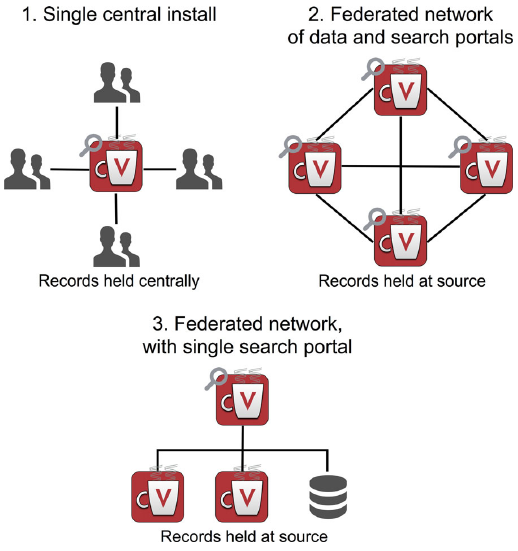
\includegraphics[width=.5\linewidth]{cafevariome-network.png}
    \caption{The available network architectures in Cafe Variome. Image retrieved from~\cite{cafevariome}.}
\end{figure}

Despite the chosen arrangement, each node can choose to customize the access policies for specific records or fields, making them available for discovery to certain groups in the network.

\subsection*{GAAIN}
One more tool analyzed because of its metadata sharing network its \gls{gaain}~\cite{gaain}, in which its main objective is to organize a community for sharing Alzheimer's-related from diverse repositories around the world, where data from different medical fields are combined together, taking into account existing policies of these repositories and preserving the ownership of the data being shared.

The architecture of \gls{gaain} contains a central server that interacts with multiple client nodes, which are installed in the data partners site (\gls{dpc}).
These \gls{gaain} \gls{dpc}s do not gather data directly from their data partner production environment, instead, data is locally exported, transformed into a CSV file and only then loaded into the \gls{dpc}.
With this process a \gls{dpc} will have a low footprint, not interfering with the data parters system, and also is given the freedom to the data owners to update their data when they find it convenient.
To have this \gls{dpc} running on the data partner's site, the only requirement imposed is to adapt current firewall configurations to allow incoming HTTPS traffic from the central server into their network.
Data owners still have full control over their data, and to do so every \gls{gaain} \gls{dpc} has ``on/off switch'' which gives the possibility to immediately detach the data from the network.

\begin{figure}[H]
    \centering
    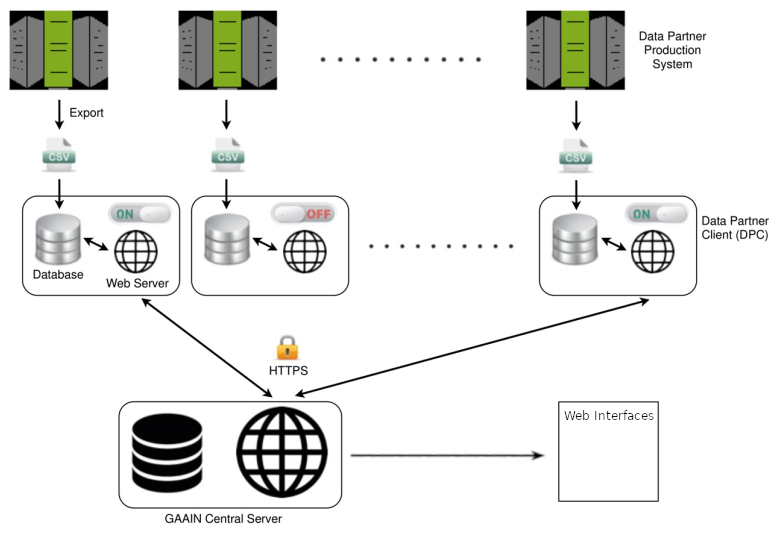
\includegraphics[width=.7\linewidth]{gaain.png}
    \caption{Network architecture of the \gls{gaain}. Image created based on an original retrieved from~\cite{gaain}.}
\end{figure}

Then, with this network architecture, \gls{gaain} researchers can query the network through its web interfaces, which forwards the search requests to the central server component which then queries every individual \gls{dpc}.
The results are sent back to the central server that aggregates them into a response to then be displayed on the web interface.

\subsection*{PopMedNet}
With the increase of availability of electronic health information, the engagement to distributed health data research networks has risen.
Popmednet~\cite{popmednet} appears to facilitate the creation and management of distributed health networks, taking into account the demands of different data owners and researchers.
The platform's adaptable architecture allows network designs that satisfy important requirements of data owners of a network, including data privacy, security requirements and network monitoring functionalities.
Researchers have available a set of features that aid in the processes of finding possible data owner collaborators, finding previously carried out research and learn more about the data in the network, thus the system is going beyond of just issuing queries.

The platform is made of two components: a web-based portal for issuing research requests and managing the network, and the clients' DataMart.
They communicate with each other following a publish-subscribe philosophy, which removes the need for data owners to have open ports on their systems, solving an important security concern of existing direct external access to local data.
With this approach, the DataMart Client is present at the data owner's local machine, behind their firewall, and all queries from the network portal are pulled from it, instead of them being pushed through an open port.
Data owners can then use the DataMart Client to review requests fetched from the network portal by analyzing its metadata such as information of the requester and the description and purpose of the request.
Then it can opt to execute the query and send the results back to the network portal, keep it for additional review or refuse it.
With this asynchronous approach to querying, data owners have full control of their data and all its uses, however, instead of doing these review steps manually, it is also given the possibility to automate them.

\subsection*{EHR4CR}
Yet another project with an interesting network design to share \gls{ehr} is the EHR4CR~\cite{ehr4cr} project.
It aims to create a robust and scalable platform to share data from distributed \gls{cdw}, taking into account requirements and policies, such as data protection, allowing to identify patient cohorts (a group of patients that satisfy specific criteria) and to extract patient-centric data.

The access to the clinical data present at each \gls{cdw} endpoint is done through three logical layers:
\begin{itemize}
    \item Legacy system layer: specific to the \gls{cdw};
    \item Legacy Interface layer: deals with the complexity of translating queries against the EHR4RC data model to the terminology used by the specific \gls{cdw} or \gls{ehr} system and also convert the results of such queries to the common EHR4RC data model;
    \item EHR4CR Data source Endpoint layer: exposes a standard EHR4CR endpoint interface so other EHR4CR services can easily access the \gls{cdw} or \gls{ehr} system's data.
\end{itemize}
Once these layers are implemented and properly working, information about the service provider is added to the central registry of the platform, allowing users to discover and browse through them.

The platform's architecture was built around the Protocol Feasibility Scenario (PFS), which retrieved aggregated results from each data source about quantities of patients that fulfill a certain Eligibility Criteria (EC), and the Patient identification and Recruitment Scenario, that has the goal of retrieving patient information with consent to furder be used on research.
The most important scenario to analyze is the PFS one, where makes use of three main components:
\begin{itemize}
    \item Workbench: acts as an interface where an end-user can issue EC queries to execute on the network and see the aggregated results;
    \item Orchestrator: distributes the queries received from the workbench across the data endpoints of the network, joining the returned results and sending them back to the workbench;
    \item Endpoint: services with \gls{cdw}s where the queries will execute.
\end{itemize}

\begin{figure}[H]
    \centering
    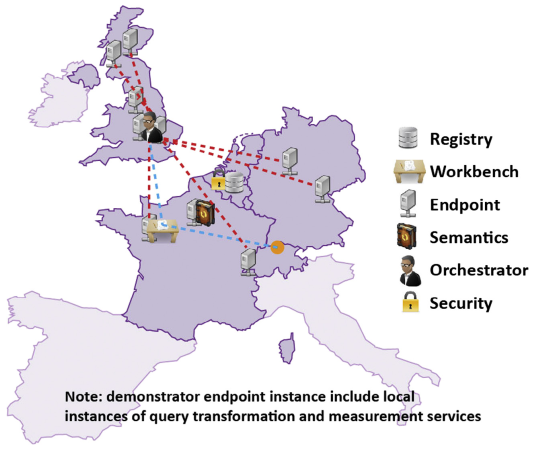
\includegraphics[width=.7\linewidth]{ehr4cr.png}
    \caption{Interation between the main services used on the Protocol Feasibility Scenario. Image retrieved from~\cite{ehr4cr}.}
\end{figure}

While building the platform, data owners' common security policies and firewall restrictions were taken into account by supporting the invocation of web services using dynamically configurable transport bindings.
Examples of such are publish-subscribe methods that were mentioned in the previous tool, where an endpoint retrieves (pull) incoming queries instead of receiving them directly (push).
This guarantees agreement to local data owners' security policies, without jeopardizing existing authentication and authorization mechanisms on end-user and web service clients.

\subsection*{NextGen Connect}
% User guide - https://www.nextgen.com/-/media/files/nextgen-connect/nextgen-connect-310-user-guide.pdf
%https://github.com/nextgenhealthcare/connect
Data owners face challenges when trying to share vital patient data quickly since institutions are pressured to keep interoperability a secure cost-effective functionally.
To do so, IT administrators need solutions that allow customization and are scalable.

In a continuously changing healthcare economy, NextGen Healthcare Solutions assist in supersede these challenges by: increasing the capabilities of sharing data; efficiently combine and transfer data over multiple systems; diminish costs and satisfy urging needs with Fast Healthcare Interoperability Resources (FHIR, a standard that defines data formats and API to exchange \gls{ehr} ) based APIs.
One of such solutions is NextGen Connect, where NextGen Healthcare's goal is to offer the healthcare society a secure and practical way to share health data.

NextGen Connect\cite{nextgen} contains an Integration Engine that, like a language interpreter who translates from one language into another, translates a message represented on a given format into another that the destination system understands.
Whenever NextGen Connect receives a message from an external system, the Integration Engine perform:
\begin{itemize}
    \item Filtering: analyses the message parameters and transfers or discards it from going to the transformation phase;
    \item Transformation: converts the message from its original format to the desired standard format (e.g., HL7 to XML) (Popular Medical standards supported, ex: DICOM, HL7). The tool also allows more customizable transformations by executing custom Javascript or Java code;
    \item Extraction: retrieve data from and send to a database;
    \item Routing: ensure that all messages are received by their destinations.
\end{itemize}
The components that are configured and execute the jobs mentioned above are called channels.
It consists of multiple connectors which are in charge of loading the data into NextGen Connect (source connector) or loading the data to an outside system (destination connector).
Each channel has exactly one source connector and one or more destination connectors.
A possible configuration is to receive data over HTTP, then send the result of the configured transformations to a file and/or insert it into a configured database.

\section{Summary}

\begin{table}
    \center
    \begin{tabular}{|*{6}{c |}}
\hline
        \multirow{2}{*}{Tool Name} & \multirow{2}{*}{Open Source} & \multicolumn{2}{c|}{Visualization/Interaction} & \multirow{2}{*}{Extraction} & \multirow{2}{*}{Network} \\
\cline{3-4}
        & & Data protection  & FAIR & &   \\
\hline
        eGenVar \cite{egenvar} & {\color{green} \cmark} \repo{https://github.com/Sabryr/EGDMS} & {\color{green} \cmark} (Users + Permissions)& {\color{green} \cmark} & {\color{red} \xmark} & {\color{red} \xmark} \\
\hline
        MONTRA \cite{montra} & {\color{green} \cmark} \repo{https://github.com/bioinformatics-ua/montra} & {\color{green} \cmark} (Role based) & {\color{green} \cmark} & {\color{red} \xmark} &  {\color{red} \xmark} \\
\hline
        REDCap \cite{redcap} & {\color{red} \xmark} & {\color{green} \cmark} (Role based) & {\color{green} \cmark} & {\color{red} \xmark} & {\color{red} \xmark}  \\
\hline
        Data Sphere \cite{datasphere} & {\color{red} \xmark} & {\color{green} \cmark} (Authorized Users Only) & {\color{red} \xmark} & {\color{red} \xmark} & {\color{red} \xmark} \\
\hline
        MOLGENIS \cite{molgenis} & {\color{green} \cmark} \repo{https://github.com/molgenis/molgenis} & {\color{green} \cmark} (Role based) & {\color{green} \cmark} & {\color{red} \xmark} & {\color{red} \xmark} \\
\hline
        Cafe Variome \cite{cafevariome} & {\color{red} \xmark} & {\color{green} \cmark} (Role based) & {\color{green} \cmark} & {\color{red} \xmark} & {\color{green} \cmark} \\
\hline
        Mica \& Opal \cite{mica} & {\color{green} \cmark} \repo{https://github.com/obiba/mica2} & {\color{red} \xmark} & {\color{green} \cmark} & {\color{red} \xmark} & {\color{red} \xmark} \\
\hline
        BioSharing \cite{biosharing} & {\color{green} \cmark} \repo{https://github.com/FAIRsharing/fairsharing.github.io/} & {\color{red} \xmark} & {\color{green} \cmark} & {\color{red} \xmark} & {\color{red} \xmark} \\
\hline
        Dataverse \cite{dataverse} & {\color{green} \cmark} \repo{https://github.com/IQSS/dataverse} & {\color{green} \cmark} (Role Based) & {\color{green} \cmark} & {\color{red} \xmark} & {\color{red} \xmark} \\
\hline
        NADA \cite{nada} & {\color{green} \cmark} \repo{https://github.com/ihsn/nada} & {\color{green} \cmark} (Access Request) & {\color{red} \xmark} & {\color{red} \xmark} & {\color{red} \xmark} \\
\hline
\hline
        ACHILLES \cite{achilles-github} & {\color{green} \cmark} \repo{https://github.com/OHDSI/Achilles/} & \multicolumn{2}{c|}{\color{red} \xmark} & {\color{green} \cmark} & {\color{red} \xmark} \\
\hline
        DataMed \cite{datamed} & {\color{green} \cmark} \repo{https://github.com/biocaddie} & \multicolumn{2}{c|}{\color{red} \xmark} & {\color{green} \cmark} & {\color{red} \xmark} \\
\hline
        %MetaExtractor \cite{metaextractor} & {\color{red} \xmark} & \multicolumn{2}{c|}{\color{red} \xmark} & {\color{green} \cmark} & {\color{red} \xmark} \\
%\hline
        Xtract \cite{xtract} & {\color{red} \xmark} & \multicolumn{2}{c|}{\color{red} \xmark} & {\color{green} \cmark} & {\color{green} \cmark} \\
\hline
        Skluma \cite{skluma} & {\color{green} \cmark} \repo{https://github.com/globus-labs/skluma-local-deploy} & \multicolumn{2}{c|}{\color{red} \xmark} & {\color{green} \cmark} & {\color{red} \xmark} \\
\hline
\hline
        GAAIN \cite{gaain} & {\color{red} \xmark} & \multicolumn{2}{c|}{\color{red} \xmark} & {\color{red} \xmark} & {\color{green} \cmark} \\
\hline
        PopMedNet \cite{popmednet} & {\color{red} \xmark} & \multicolumn{2}{c|}{\color{red} \xmark} & {\color{red} \xmark} & {\color{green} \cmark} \\
\hline
        EHR4CR \cite{ehr4cr} & {\color{red} \xmark} & \multicolumn{2}{c|}{\color{red} \xmark} & {\color{red} \xmark} & {\color{green} \cmark} \\
\hline
        NextGen Connect \cite{nextgen} & {\color{green} \cmark} \repo{https://github.com/nextgenhealthcare/connect} & \multicolumn{2}{c|}{\color{red} \xmark} & {\color{red} \xmark} & {\color{green} \cmark} \\
\hline
\end{tabular}
    \caption{A summary of the features present in each tool studied in this Background chapter.}
    \label{tab:background-resumo}
\end{table}

In this chapter, several tools were analyzed regarding metadata visualization, extraction, and tools implementing networks of metadata.
Table \ref{tab:background-resumo} enumerates all the tools analyzed, as well as, marked with a green check, features that the specific tool supports and marked with a red cross, not supported features.
It is possible to see that no tool contains all the desired features.
It is then required to either build a system that supports all these features or make integration of a set of these tools.

Either way, this study will help on further development processes, due to the aspects that certain tools might alert to, such as, on \cite{popmednet}, software running on the local environment of the data owners followed a pull approach for communication instead of push, to avoid requiring open ports on their systems, which could lead to having to change critical firewall rules.
Also, on \cite{gaain}, it was given the possibility to data owners to deactivate software related to the \gls{gaain} project running on their local system.
Furthermore, one interesting fact that extraction tools had in common, was that either the data was assumed to be or was first transformed into a common format before performing any extraction processes.

Both \cite{montra} and \cite{achilles-github} look promising to be used on this work, due to its database-centric design and also for already being used on the \gls{ehden} project.
However, there is still the need for a system that gets the data from the agents extracting the data to the applications holding and displaying the data.

The next chapter will approach the platform that will be used to store and visualize the metadata, detailing its features and consequential improvements.
